% !TeX program = pdflatex
% !BIB program = biber
\documentclass{fhnwreport}
\usepackage[english,nswissgerman]{babel}
\usepackage[T1]{fontenc}
\usepackage[utf8]{inputenc}
\usepackage{lmodern}
\usepackage{textcomp}
\usepackage{graphicx}
\usepackage{float}
\usepackage[dvipsnames]{xcolor}
\usepackage{csquotes}
\usepackage{amsmath,amssymb}
\usepackage{siunitx}
\usepackage{booktabs,tabularx,longtable}
\usepackage{listings}
\usepackage[bottom]{footmisc}
\usepackage{pdfpages,pdflscape}
\usepackage{microtype}

\graphicspath{{graphics/}}
\sisetup{locale=DE}
\urlstyle{same}

\newcolumntype{L}[1]{>{\raggedright\arraybackslash}p{#1}}
\newcolumntype{C}[1]{>{\centering\arraybackslash}p{#1}}
\newcolumntype{R}[1]{>{\raggedleft\arraybackslash}p{#1}}

% Sichtbare Arbeitsnotizen beim Ausarbeiten durch den eigentlichen Text ersetzen.
\newcommand{\arbeitsnotiz}[1]{\par\noindent{\color{gray}\itshape #1}\par}

\lstset{
  language=Python,
  basicstyle=\ttfamily\small,
  breaklines=true,
  showstringspaces=false,
  columns=fullflexible,
  frame=single,
  captionpos=b
}


\newcommand{\logofilename}{FHNW_HTU_DE}
\newcommand{\projektteam}{Zephyr Kesseler, Damian Szedalik}
\newcommand{\abgabedatum}{[Abgabedatum ergänzen]}

\usepackage[backend=biber,style=apa,sortlocale=de_CH]{biblatex}
\addbibresource{literature/literatur.bib}

\title{Athletes Network\\Soziale Netzwerkanalyse im Schwimmsport}
\author{Projektarbeit im Modul Soziale Netzwerke}
\date{\abgabedatum}
\hypersetup{
  pdftitle={Athletes Network: Soziale Netzwerkanalyse im Schwimmsport},
  pdfauthor={\projektteam},
  pdfsubject={Projektarbeit im Modul Soziale Netzwerke}
}

\begin{document}
\selectlanguage{nswissgerman}
\pagenumbering{roman}
\maketitle
\vfill
\begin{tabularx}{\textwidth}{@{}lX@{}}
  Projektteam & \projektteam \\[2ex]
  Modul & Soziale Netzwerke \\[2ex]
  Studiengang & Data Science \& AI \\[2ex]
  Hochschule & Fachhochschule Nordwestschweiz
\end{tabularx}
\vfill
\clearpage

% !TeX root = ../main.tex
\section*{Zusammenfassung}
\thispagestyle{empty}
\arbeitsnotiz{Zum Abschluss Fragestellung, Datenbasis, Vorgehen und die wichtigsten Ergebnisse in einem kurzen Absatz zusammenfassen.}

\tableofcontents
\clearpage
% Aktivieren, sobald entsprechende Abbildungen und Tabellen vorhanden sind.
% \listoffigures
% \listoftables
% \clearpage

\pagenumbering{arabic}
% Dateinummern ab 03 entsprechen dem Skript. Reportnummern entstehen automatisch.
% \input vermeidet einen erzwungenen Seitenwechsel bei jedem kurzen Abschnitt.
% !TeX root = ../main.tex
\section{Einleitung}
\label{sec:einleitung}

\subsection{Ausgangslage und Ziel}
\arbeitsnotiz{Thema und Erkenntnisinteresse beschreiben. Kurz erläutern, welchen zusätzlichen Blick eine Netzwerkanalyse auf die Schwimmdaten ermöglicht.}

\subsection{Fragestellungen}
\arbeitsnotiz{Die ausgewählten Fragestellungen präzise formulieren und den Untersuchungsrahmen abgrenzen.}

% !TeX root = ../main.tex
\section{Datenbeschaffung und explorative Datenanalyse}
\label{sec:daten}

\subsection{Datenquelle und Erhebung}
Der verwendete Scraper entstand 2025 im Rahmen eines anderen Projekts. Mit
Python und Selenium wurden Mitte 2025 auf
\href{https://www.swimrankings.net}{swimrankings.net} die TOP100 Listen mit
bis zu 100 Männern und 100 Frauen je Land sowie deren persönliche
Bestleistungen erfasst. Die vorliegende
Arbeit verwendet diese gespeicherten Rohdaten weiter. Eine Zeile entspricht
einem Bestleistungseintrag und verbindet Athletenmerkmale wie Jahrgang,
Geschlecht, Nation und Verein mit Disziplin, Beckenlänge, Zeit, Punkten sowie
Datum, Ort und Wettkampfname.

Das Land der ausgewählten Liste (Listenland) kann von der Nation im
Athletenprofil (Profilnation) abweichen. Beispielsweise erscheinen Athleten
mit spanischer Profilnation auch auf portugiesischen Listen. Beim
Zusammenführen aller Länderlisten können deshalb mehr als 200 Personen
derselben Profilnation im Datensatz enthalten sein.

Ein ergänzendes Skript sollte 126 vermutete Erhebungsausfälle nachladen.
Bei diesen Profilen fehlten sowohl Bestleistungen als auch Detailangaben.
Der im EDA Notebook dokumentierte Versuch scheiterte an Cloudflare
Prüfungen, obwohl das Skript mit einer manuellen Prüfung im Browser durchgeführt wurde. Es wurden dadurch keine zusätzlichen Daten gewonnen.

\subsection{Bereinigung und Datenqualität}
Entfernt wurden 1\,688 Zeilen ohne Bestleistungen von 1\,687 Athleten,
134 exakte Duplikate und der unplausible Quellenwert \texttt{55:55.55}
über 200\,m Brust. Fehlende Bestleistungen gelten dabei nicht grundsätzlich
als Erhebungsfehler. Zeiten wurden in Sekunden umgerechnet, Datentypen
vereinheitlicht und fehlende Angaben erkennbar belassen. Fehlende Orte und
Wettkampfnamen sind als \texttt{Unknown} markiert. Die kombinierte Profilangabe
wurde in Nation und Verein aufgeteilt. Listenland und Profilnation bleiben
erhalten, da sie bei 215 Athleten voneinander abweichen.

Quellenstichproben und Plausibilitätsprüfungen ergänzten die Bereinigung.
Die auffälligen ungefähren Alterswerte von 6 und 66 Jahren wurden bestätigt und
beibehalten. Der Parquet Export wurde erneut eingelesen und auf
Übereinstimmung mit der bereinigten Tabelle geprüft. Tabelle~\ref{tab:datenumfang}
zeigt den resultierenden Datenumfang. Die einzelnen Prüfungen sind in
\nolinkurl{Notebooks/01_eda.ipynb} dokumentiert.

\begin{table}[H]
  \centering
  \caption{Datenumfang vor und nach der Bereinigung. Eigene Auswertung.}
  \label{tab:datenumfang}
  \begin{tabular}{@{}lrr@{}}
    \toprule
    Datenstand & Zeilen & Athleten \\
    \midrule
    Rohdaten & 286\,996 & 14\,849 \\
    Bereinigt & 285\,173 & 13\,162 \\
    \bottomrule
  \end{tabular}
\end{table}

\subsection{Erkenntnisse und Grenzen}
Für die Auswertung nach Nation zählt jede Athletenkennung einmal und wird
der Profilnation zugeordnet. Die 13\,162 Athleten verteilen sich auf
182 Profilnationen. Die Abdeckung
reicht von einer bis zu 218 Personen pro Nation, der Median beträgt nur 28.
Männer machen 55,7\,\% und Frauen 44,3\,\% aus. Die 126 vermuteten
Erhebungsausfälle betreffen 122 Frauen und 4 Männer. Länderanalysen und
Geschlechtervergleiche können dadurch verzerrt sein. Bei den bekannten
Geburtsjahrgängen liegt der Median bei 1997, die mittleren 50\,\% liegen
zwischen 1989 und 2002.

Pro Athlet sind im Median 19 Bestleistungseinträge gespeichert, die mittleren
50\,\% umfassen 9 bis 34 Einträge. Einzelne Personen sind damit deutlich
umfangreicher dokumentiert als andere. Die Leistungen verteilen sich mit
52,0\,\% auf die Langbahn (50\,m) und mit 48,0\,\% auf die Kurzbahn (25\,m).
Neben vollständigen Strecken sind auch Zwischenzeiten mit dem Zusatz
\texttt{Lap} enthalten.

Die datierten Einträge reichen vom 17. Oktober 1964 bis zum 8. April 2025.
Davon stammen 94,7\,\% aus den Jahren ab 2005. Abbildung~\ref{fig:eda}
zeigt den lokalen Anstieg 2009 und den Einbruch 2020. Ursachen lassen sich
daraus allein nicht ableiten. Das Jahr 2025 ist nur teilweise erfasst und
daher nicht direkt mit vollständigen Jahren vergleichbar. Für die weitere
Modellierung bleiben alle Jahre erhalten.

\begin{figure}[H]
  \centering
  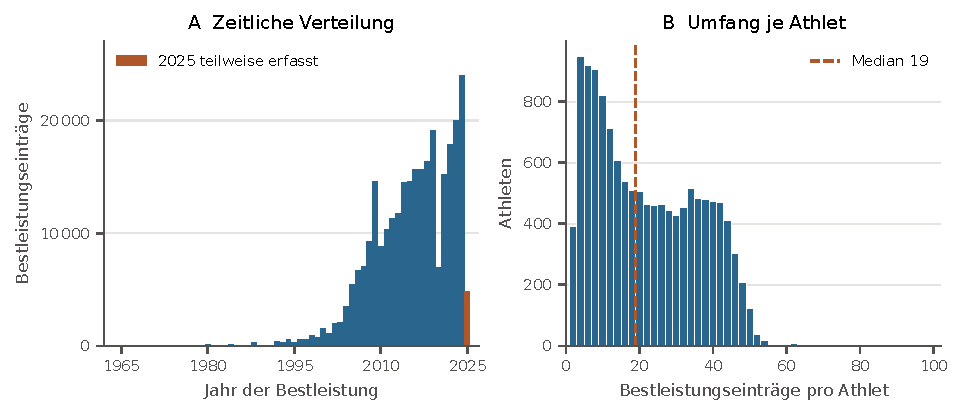
\includegraphics[width=\textwidth]{02_eda_ueberblick.pdf}
  \caption{Zeitliche Verteilung und Umfang der gespeicherten Bestleistungen.
  Links fehlt ein Eintrag ohne Datum. Rechts zählt jeder Athlet einmal.
  Eigene Auswertung.}
  \label{fig:eda}
\end{figure}

Bei 5\,115 Athleten (38,9\,\%) fehlen Vereinsangaben. Auch die Punkte sind
nicht vollständig: Von 53\,577 Einträgen ohne Punkte entfallen 53\,019 auf
\texttt{Lap} und 558 auf seltene Kombinationen aus Disziplin und Beckenlänge.
Diese Lücken bestehen bereits in der Quelle und häufen sich somit bei
bestimmten Leistungsarten.

Die Auswahl über TOP100 Listen und persönliche Bestleistungen bildet weder
den gesamten Schwimmsport noch vollständige Wettkampfbiografien ab. Die
Häufigkeiten beschreiben gespeicherte Bestleistungen und erlauben keine
direkten Aussagen zur Anzahl aller Wettkampfteilnahmen. Gekürzte und
wiederholte Wettkampfnamen bleiben erhalten, sind für sich allein aber keine
eindeutigen Veranstaltungskennungen. Die Datenbasis bleibt auf dem
Erhebungsstand von 2025.

% !TeX root = ../main.tex
\section{Modellierung}
\label{sec:modellierung}

\arbeitsnotiz{Die Modellwahl wird gemeinsam neu festgelegt. Anschliessend werden Fragestellung, Knoten, Kanten, Gewichtung und die wichtigsten Grenzen knapp beschrieben. Die Netzwerktypen aus Kapitel~3 des Skripts dienen als Grundlage \parencite{henninger2024}.}

% !TeX root = ../main.tex
\section{Reduktion des Netzwerks}
\label{sec:reduktion}
\arbeitsnotiz{Einen begründeten Analyseumfang wählen. Falls eine Filterung nötig ist, Kriterium und verbleibende Knoten und Kanten nennen. Die grösste Zusammenhangskomponente nur für Analysen verwenden, die dies benötigen.}

% !TeX root = ../main.tex
\section{Communities}
\label{sec:communities}
\arbeitsnotiz{Communities mit einem passenden Verfahren untersuchen, etwa Louvain. Eine Abbildung und die Zusammensetzung ausgewählter Gruppen anhand der Profilnation oder Disziplinen interpretieren.}

% !TeX root = ../main.tex
\section{Wichtigkeit von Knoten}
\label{sec:zentralitaet}
\arbeitsnotiz{Degree und Betweenness als zwei unterschiedliche Rollen vergleichen. Wenige auffällige Athleten erklären und die gewählte Behandlung der Kantengewichte nennen. Keine vollständige Rangliste aller Zentralitätsmasse erstellen.}

% % !TeX root = ../main.tex
% Optional. In main.tex nur bei einem sinnvollen Vergleich aktivieren.
\section{Netzwerkzentralisierung}
\label{sec:zentralisierung}
\arbeitsnotiz{Nur ergänzen, wenn eine Zentralisierung zusätzliche Erkenntnisse über vergleichbare Teilnetze liefert. Andernfalls entfällt dieser Abschnitt.}

% !TeX root = ../main.tex
\section{Netzwerkmetriken}
\label{sec:netzwerkmetriken}
\arbeitsnotiz{Grösse, Zusammenhangskomponenten, Dichte und Clustering in einer kompakten Übersicht einordnen. Dabei beachten, dass gemeinsame Wettkampftage bei der Projektion bereits Dreiecke erzeugen.}

% !TeX root = ../main.tex
\section{Konnektivität}
\label{sec:konnektivitaet}
\arbeitsnotiz{Als kleinen Robustheitsvergleich denselben Anteil besonders zentraler beziehungsweise zufälliger Athleten entfernen. Die Veränderung der grössten Zusammenhangskomponente vergleichen, Zufallsentnahmen wiederholen und als Simulation interpretieren.}

% !TeX root = ../main.tex
\section{Korrelation in Netzwerken}
\label{sec:korrelation}
\arbeitsnotiz{Mit der Assortativität untersuchen, ob verbundene Athleten häufig dieselbe Profilnation haben. Auswahl über Länderranglisten und Erhebungslücken bei der Interpretation berücksichtigen. Die statistische Einordnung folgt im nächsten Abschnitt.}

% !TeX root = ../main.tex
\section{Inferenzielle Statistik in Netzwerken}
\label{sec:inferenzstatistik}
\arbeitsnotiz{Die Frage zur Profilnation mit einem begründeten Permutationstest vertiefen. Nullmodell, beobachteten Effekt und Unsicherheit erklären. Eine Aussage über persönliche Präferenzen lässt sich daraus nicht ableiten.}

% Optionale Vertiefungen nur bei einer passenden Fragestellung aktivieren.
% % !TeX root = ../main.tex
% Optional. In main.tex nur bei einem tragfähigen zeitlichen Experiment aktivieren.
\section{Link Prediction}
\label{sec:link_prediction}
\arbeitsnotiz{Nur bei einem belastbaren zeitlichen Aufbau ergänzen. Die Bestleistungsdaten bilden keine vollständige Folge historischer Teilnahmen ab. Eine Vorhersage müsste sich auf später erfasste Verbindungen in dieser Auswahl beschränken.}

% % !TeX root = ../main.tex
% Optional. Für den geplanten Projektumfang zunächst nicht vorgesehen.
\section{Diffusion}
\label{sec:diffusion}
\arbeitsnotiz{Nur bei einer zusätzlichen passenden Fragestellung ergänzen. Eine Simulation auf dem Bestleistungsnetzwerk wäre ein hypothetisches Szenario ohne beobachtete Übertragungen.}

% % !TeX root = ../main.tex
% Optional. Für den geplanten Projektumfang zunächst nicht vorgesehen.
\section{Graphlets}
\label{sec:graphlets}
\arbeitsnotiz{Nur ergänzen, wenn der Vergleich lokaler Strukturen einen klaren Zusatznutzen hat. Durch die Projektion erzeugte Cliquen bei der Interpretation berücksichtigen.}

% !TeX root = ../main.tex
\section{Fazit und Ausblick}
\label{sec:schluss}

\subsection{Beantwortung der Fragestellungen}
\arbeitsnotiz{Die zentralen Ergebnisse zusammenführen und die Fragen aus der Einleitung beantworten.}

\subsection{Grenzen, Ausblick und Reflexion}
\arbeitsnotiz{Die Aussagekraft einordnen, konkrete Erweiterungen nennen und kurz festhalten, was gut lief und was künftig anders gemacht würde.}


\clearpage
\printbibliography[heading=bibintoc,title=Literaturverzeichnis]
% !TeX root = ../main.tex
\section*{Eigenständigkeitserklärung}
\markboth{\MakeUppercase{Eigenständigkeitserklärung}}{\MakeUppercase{Eigenständigkeitserklärung}}

\addcontentsline{toc}{section}{Eigenständigkeitserklärung}

Ich (wir) erkläre(n) hiermit, dass ich (wir) den vorliegenden Leistungsnachweis selber und selbständig verfasst habe(n),
\begin{itemize} 
\item dass ich (wir) sämtliche nicht von mir (uns) selber stammenden Textstellen und anderen Quellen wie Bilder etc. gemäss gängigen wissenschaftlichen Zitierregeln\footnote{APA 7} korrekt zitiert und die verwendeten Quellen klar sichtbar ausgewiesen habe(n). 
\item dass ich (wir) in einer Fussnote oder einem Hilfsmittelverzeichnis alle verwendeten Hilfsmittel (KI-Assistenzsysteme wie Chatbots\footnote{z.B. ChatGPT}, Übersetzungs-\footnote{z.B. Deepl} Paraphrasier-\footnote{z.B. Quillbot} oder Programmierapplikationen\footnote{z.B. Github Copilot}) deklariert und ihre Verwendung bei den entsprechenden Textstellen angegeben habe(n).
\item dass ich (wir) sämtliche immateriellen Rechte an von mir (uns) allfällig verwendeten Materialien wie Bilder oder Grafiken erworben habe(n) oder dass diese Materialien von mir (uns) selbst erstellt wurde(n).
\item dass das Thema, die Arbeit oder Teile davon nicht bei einem Leistungsnachweis eines anderen Moduls verwendet wurden, sofern dies nicht ausdrücklich mit der Dozentin oder dem Dozenten im Voraus vereinbart wurde und in der Arbeit ausgewiesen wird. 
\item dass ich mir (wir uns) bewusst bin (sind), dass meine (unsere) Arbeit auf Plagiate und auf Drittautorschaft menschlichen oder technischen Ursprungs (Künstliche Intelligenz) überprüft werden kann.
\item dass ich mir (wir uns) bewusst bin (sind), dass die Hochschule für Technik FHNW einen Verstoss gegen diese Eigenständigkeitserklärung bzw. die ihr zugrundeliegenden Studierendenpflichten der Studien- und Prüfungsordnung der Hochschule für Technik verfolgt und dass daraus disziplinarische Folgen (Verweis oder Ausschluss aus dem Studiengang) resultieren können.
\end{itemize}

\vspace*{4ex}

[Ort ergänzen], \abgabedatum

\vspace*{4ex}

{\renewcommand{\arraystretch}{2}
\begin{tabular}{@{}>{\bfseries}ll}
Name: & [Name ergänzen]\\
Unterschrift: & \\[6ex]
Name: & [Name ergänzen]\\
Unterschrift: & \\
\end{tabular}
}

% !TeX root = ../main.tex
\appendix
\section{Ergänzende Materialien}
\label{app:materialien}
\arbeitsnotiz{Bei Bedarf zusätzliche Abbildungen, Prüfbeispiele und eine Übersicht der abgegebenen Notebooks und Graphdateien ergänzen.}

\section{Hilfsmittelverzeichnis}
\label{app:hilfsmittel}
\arbeitsnotiz{Verwendete Werkzeuge und KI Unterstützung mit Zweck, betroffenen Arbeitsschritten und den zugehörigen Prompts dokumentieren.}

\end{document}
